%%%%%%%%%%%%%%%%%%%%%%%%%%%%%%%%%%%%%%%%%
% University/School Laboratory Report
% LaTeX Template
% Version 4.0 (March 21, 2022)
%
% This template originates from:
% https://www.LaTeXTemplates.com
%
% Authors:
% Vel (vel@latextemplates.com)
% Linux and Unix Users Group at Virginia Tech Wiki
%
% License:
% CC BY-NC-SA 4.0 (https://creativecommons.org/licenses/by-nc-sa/4.0/)
%
%%%%%%%%%%%%%%%%%%%%%%%%%%%%%%%%%%%%%%%%%

%----------------------------------------------------------------------------------------
%	PACKAGES AND DOCUMENT CONFIGURATIONS
%----------------------------------------------------------------------------------------

\documentclass[
	letterpaper, % Paper size, specify a4paper (A4) or letterpaper (US letter)
	11pt, % Default font size, specify 10pt, 11pt or 12pt
]{CSUniSchoolLabReport}

\usepackage{subcaption}
\usepackage{booktabs}
\geometry{top=1cm, bottom=2.5cm} % Override margins to reduce space before title and fit figures

%----------------------------------------------------------------------------------------
%	REPORT INFORMATION
%----------------------------------------------------------------------------------------

\title{Lab 5 - Inductance} % Report title

\author{Yiran \textsc{Liu} \&  Zijin \textsc{Yang}} % Author name(s), add additional authors like: '\& James \textsc{Smith}'

%----------------------------------------------------------------------------------------

\begin{document}

\maketitle % Insert the title, author and date using the information specified above

\begin{center}
	\begin{tabular}{l r}
      Course: & ECE 106 \\
      Student Number: & Y.L. 21184901 \& Z.Y. 21196273
	\end{tabular}
\end{center}

%----------------------------------------------------------------------------------------
%	PREDICTIONS
%----------------------------------------------------------------------------------------

\section{Predictions}

\subsection{Switched Circuit without Coil}

\begin{figure}[H] % [H] forces the figure to be placed exactly where it appears in the text
	\centering % Horizontally center the figure
	
\includegraphics[width=0.4\textwidth]{{./figures/circuit without coil}.png} % Include the figure
	\caption{Switched circuit without the coil.}
\end{figure}

In an ideal circuit with resistance only, this circuit changes instantly. The function $I_R(t)$ can be defined using the Heaviside function:
\[
	\begin{aligned}
		\text{Close switch at } t=0 &: \quad I_R(t) = I_\text{max} \ H(t) \\
		\text{Open switch at } t=0 &: \quad I_R(t) = I_\text{max} \ H(-t) \\
		\text{where } H(t) &= \begin{cases}
			0 \quad (t<0) \\
			1 \quad (t>0)
		\end{cases}
	\end{aligned}
\]

\begin{figure}[H]
	\centering
	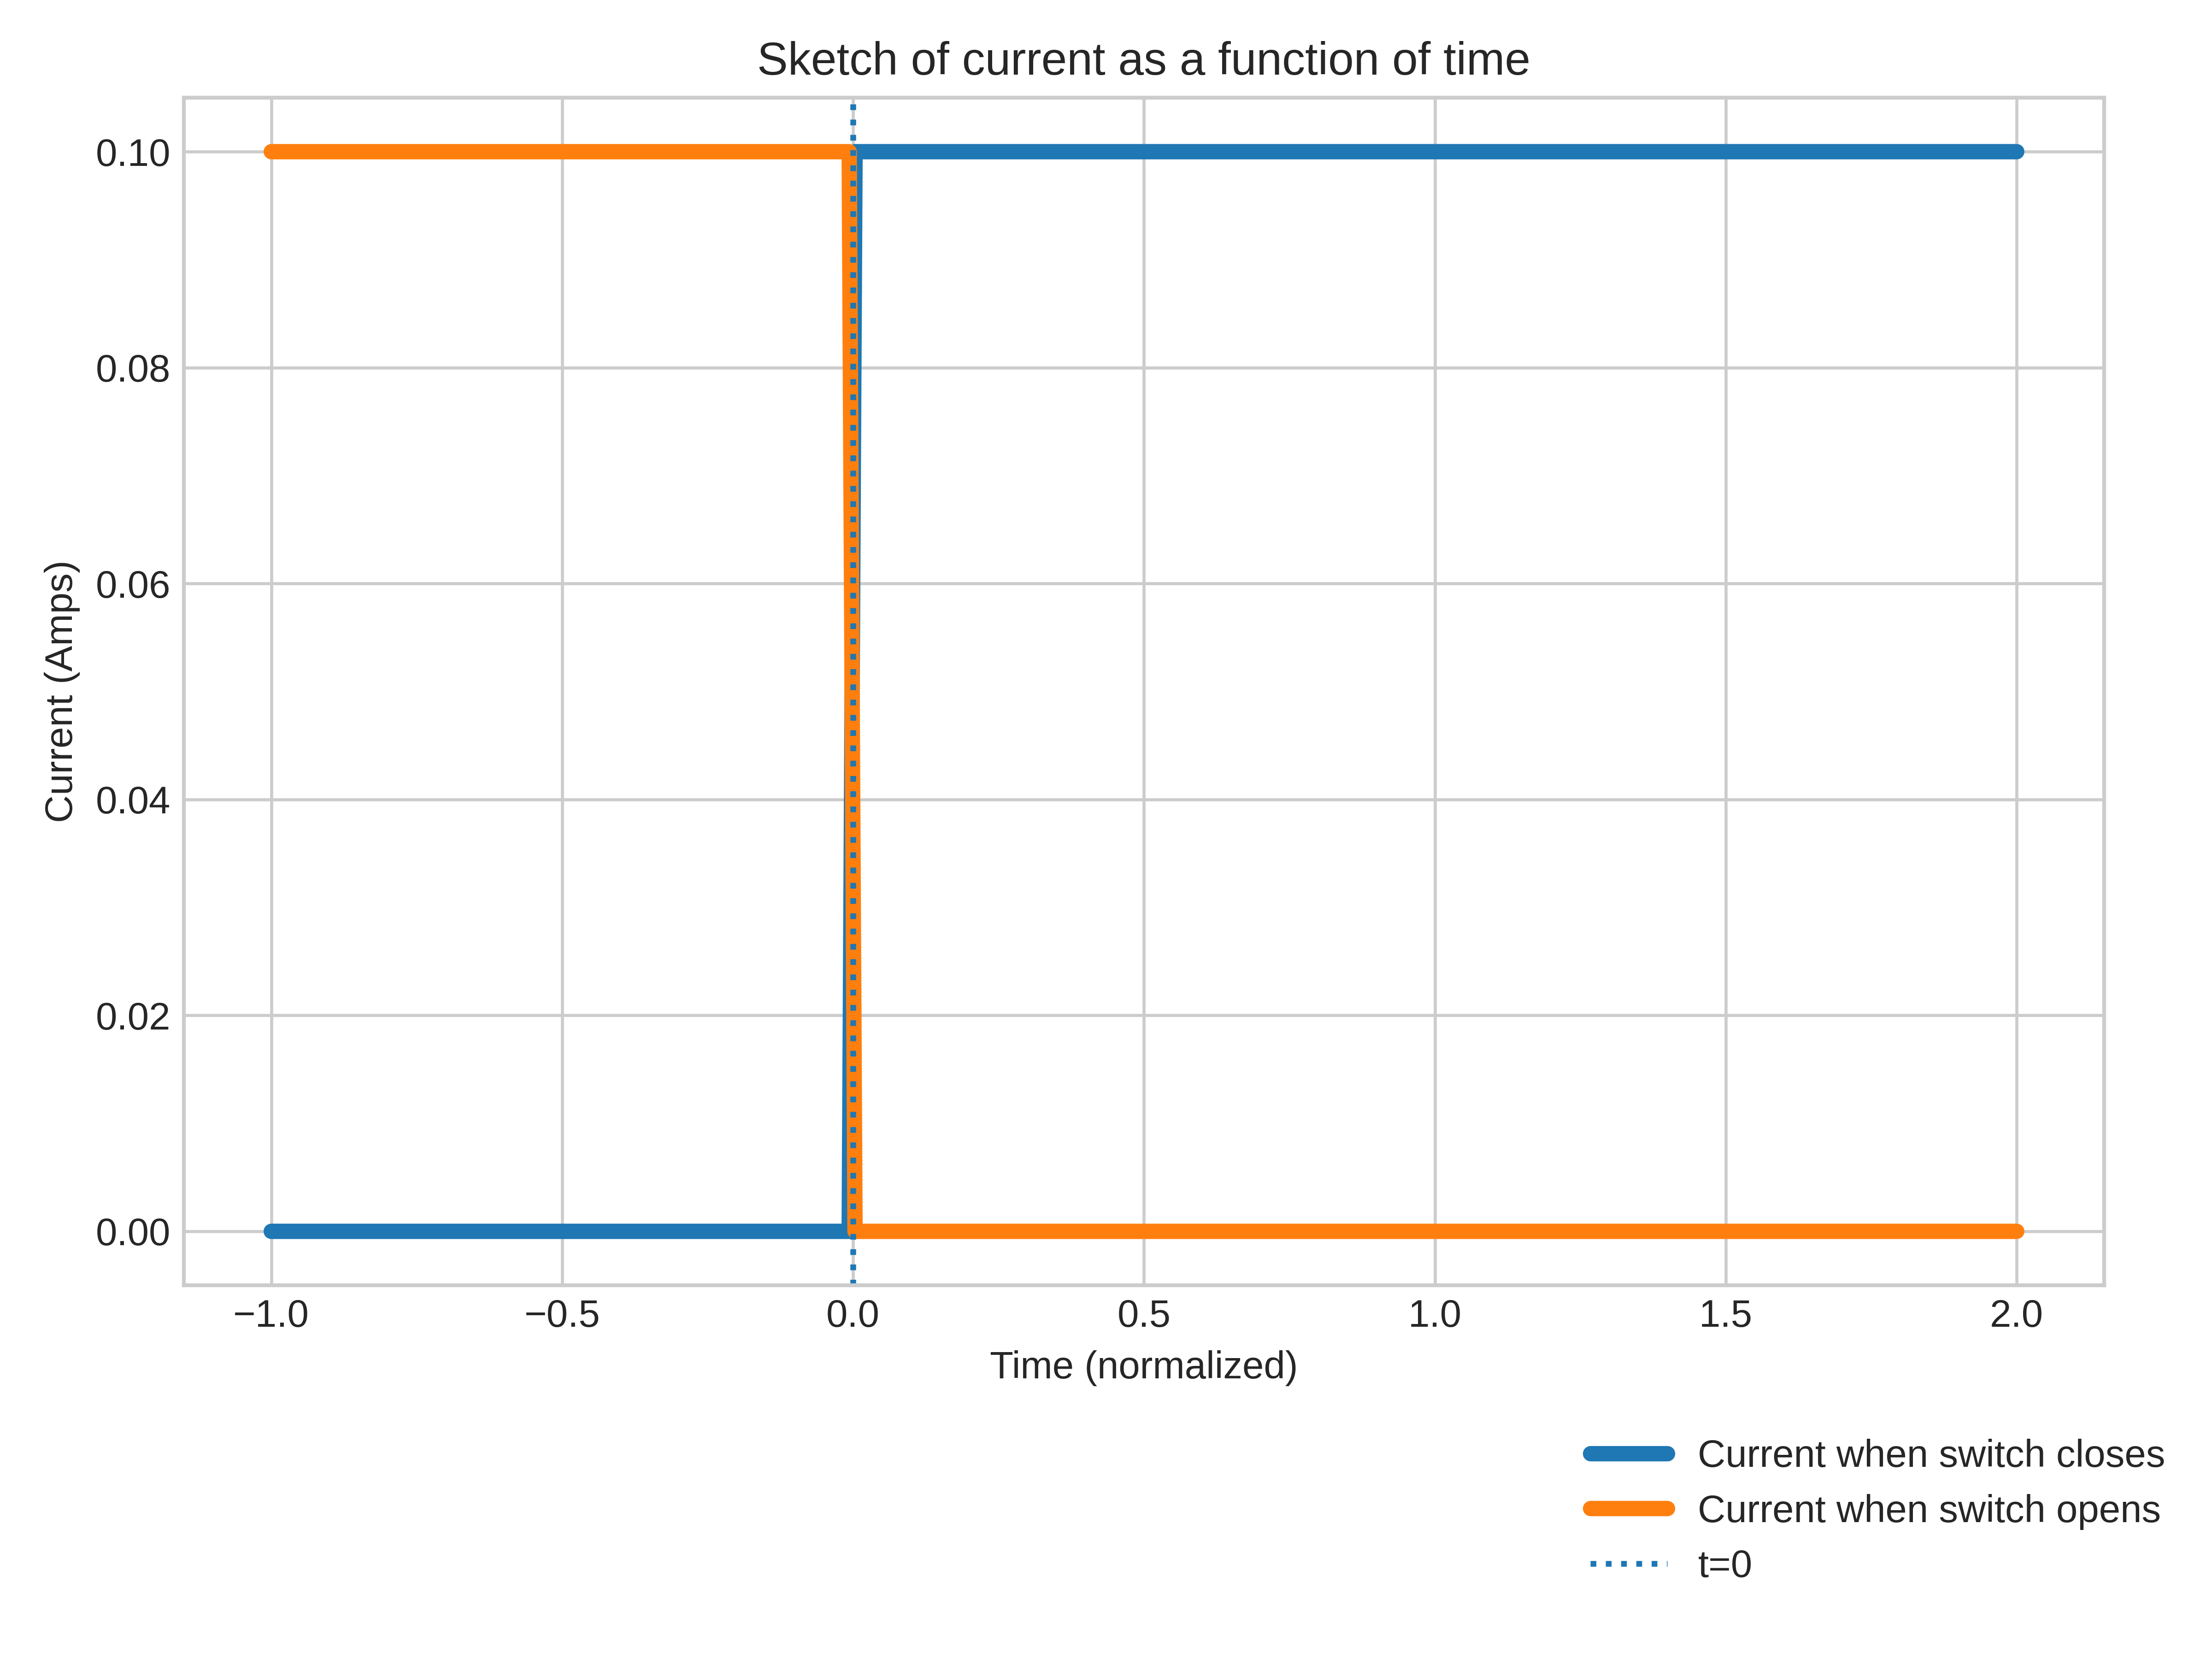
\includegraphics[width=0.75\textwidth]{./figures/current_plot_nocoil.png}
	\caption{Predicted current through the resistor without the coil.}
\end{figure}

\subsection{Switched Circuit with Coil}

\begin{figure}[H]
	\centering
	
\includegraphics[width=0.4\textwidth]{{./figures/circuit with coil}.png}
	\caption{Switched circuit with the coil.}
\end{figure}

This is a classic \textbf{L-R circuit}, therefore the charging and discharging can be described using the standard function from ECE 140:
\[
	\begin{aligned}
		\text{Close switch at } t=0 &: \quad I_R(t) = I_\text{max} \left(1-e^{-t/\tau} \right) \\
		\text{Open switch at } t=0 &: \quad I_R(t) = I_\text{max} \ e^{-t/\tau} \\
		\text{where } \tau & \text{ is the time constant.}
	\end{aligned}
\]

\begin{figure}[H]
	\centering
	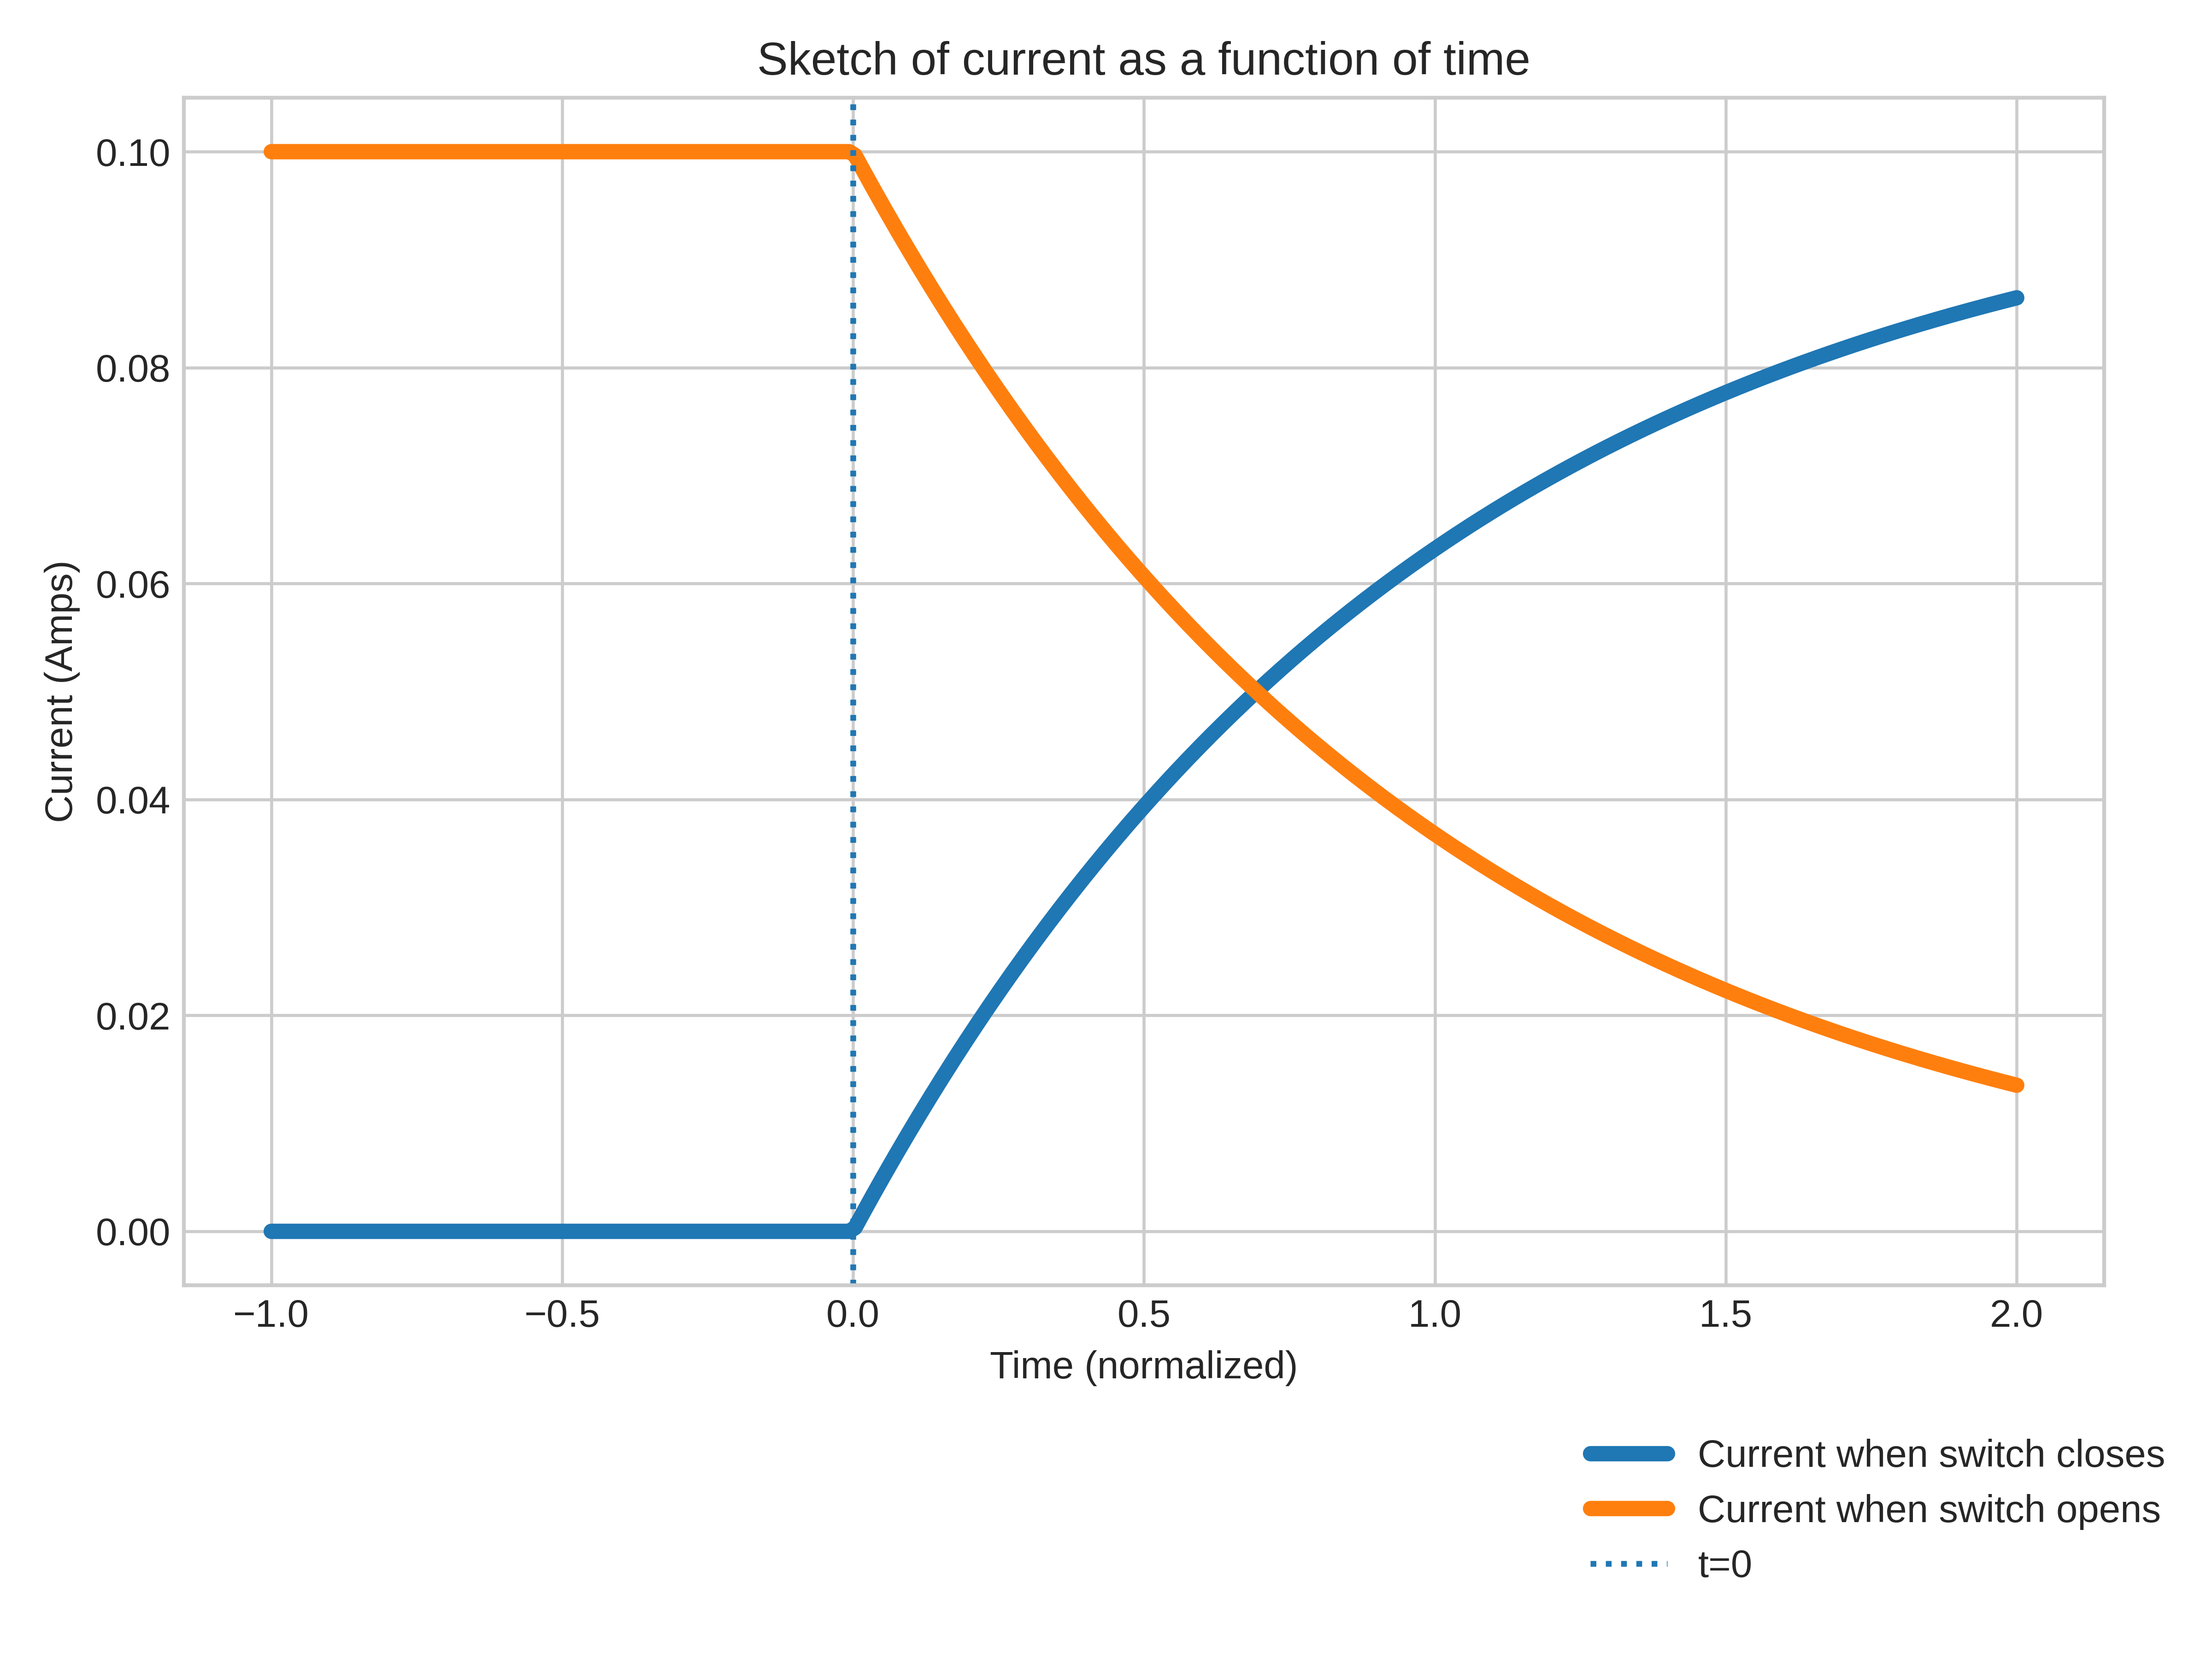
\includegraphics[width=0.75\textwidth]{./figures/current_plot_coil.png}
	\caption{Predicted current through the resistor with the coil.}
\end{figure}

\pagebreak

%----------------------------------------------------------------------------------------
%	MEASUREMENTS
%----------------------------------------------------------------------------------------

\section{Measurements}

\subsection{Rising Step Function without Coil}

\begin{figure}[H]
	\centering
	\begin{subfigure}{0.6\textwidth}
		\centering
		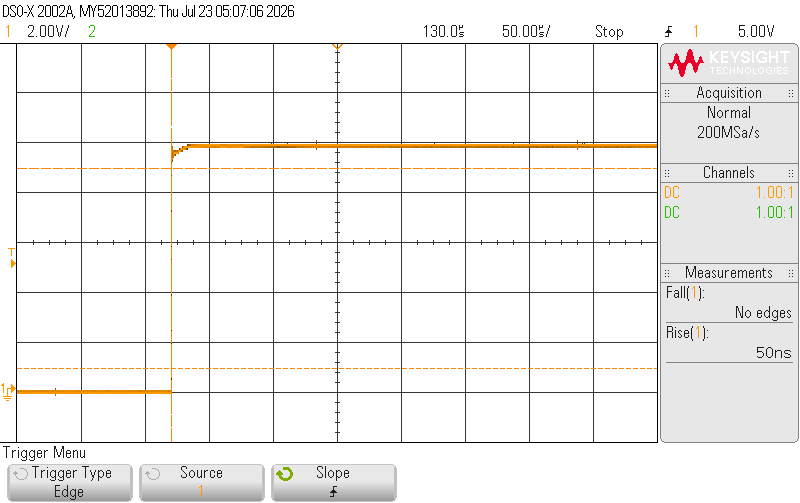
\includegraphics[width=\textwidth]{./figures/scope_0.png}
		\caption{Trial 1}
	\end{subfigure}

	\vspace{0.5em}
	\begin{subfigure}{0.6\textwidth}
		\centering
		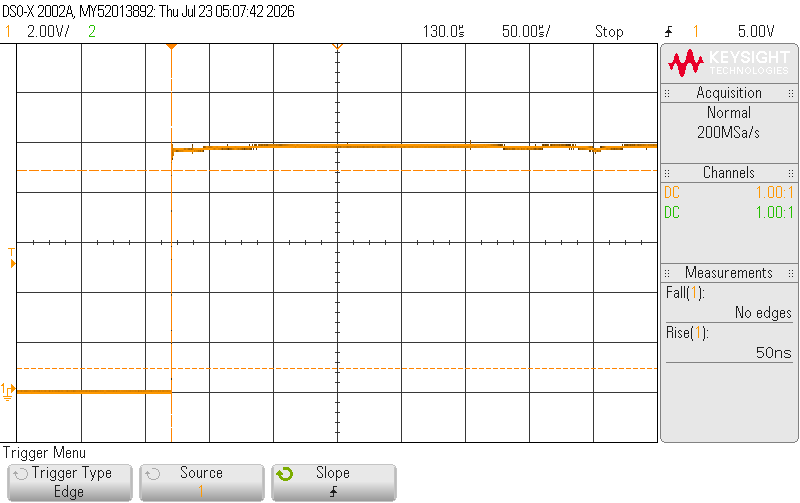
\includegraphics[width=\textwidth]{./figures/scope_1.png}
		\caption{Trial 2}
	\end{subfigure}

	\vspace{0.5em}
	\begin{subfigure}{0.6\textwidth}
		\centering
		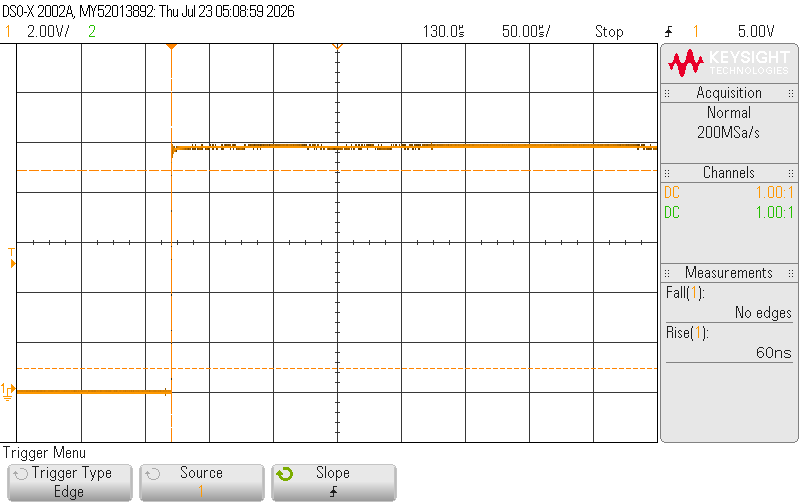
\includegraphics[width=\textwidth]{./figures/scope_2.png}
		\caption{Trial 3}
	\end{subfigure}
	\caption{Oscilloscope captures of the rising step without the coil.}
\end{figure}

\begin{table}[H]
	\centering
	\begin{tabular}{lccc}
		\toprule
		\textbf{Trial} & \textbf{1} & \textbf{2} & \textbf{3} \\
		\midrule
		Rise time & $50\,\text{ns}$ & $50\,\text{ns}$ & $60\,\text{ns}$ \\
		\bottomrule
	\end{tabular}
\end{table}

\pagebreak

\subsection{Rising Step Function with Coil}

\begin{figure}[H]
	\centering
	\begin{subfigure}{0.6\textwidth}
		\centering
		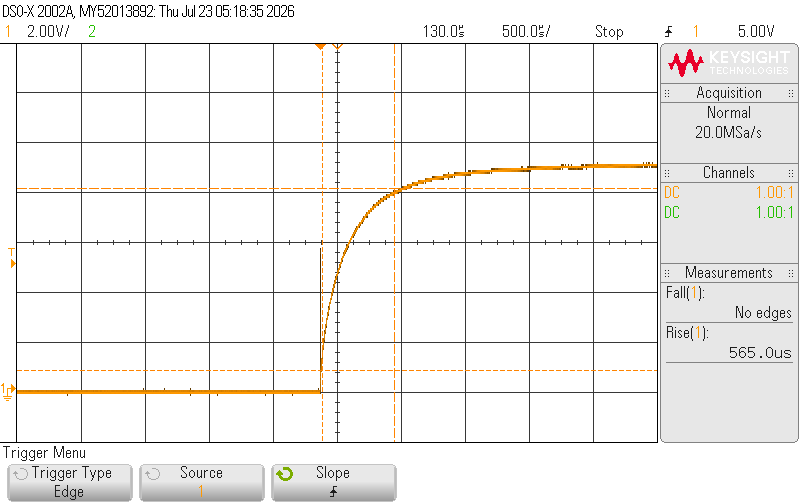
\includegraphics[width=\textwidth]{./figures/scope_3.png}
		\caption{Trial 1}
	\end{subfigure}

	\vspace{0.5em}
	\begin{subfigure}{0.6\textwidth}
		\centering
		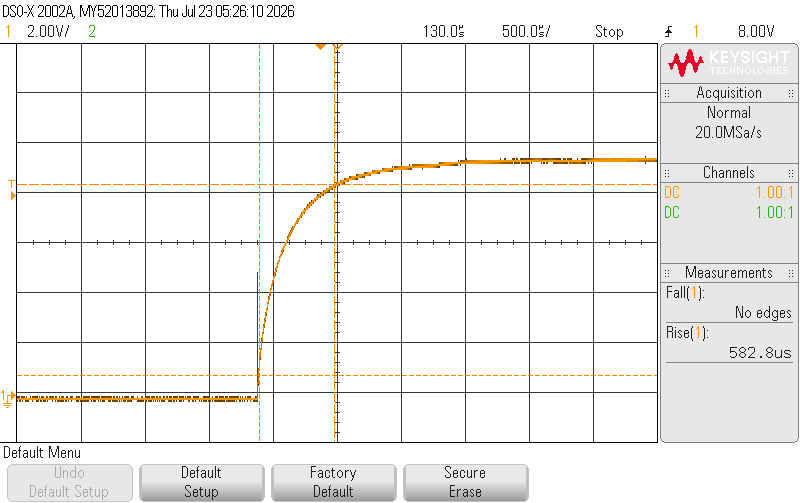
\includegraphics[width=\textwidth]{./figures/scope_4.png}
		\caption{Trial 2}
	\end{subfigure}

	\vspace{0.5em}
	\begin{subfigure}{0.6\textwidth}
		\centering
		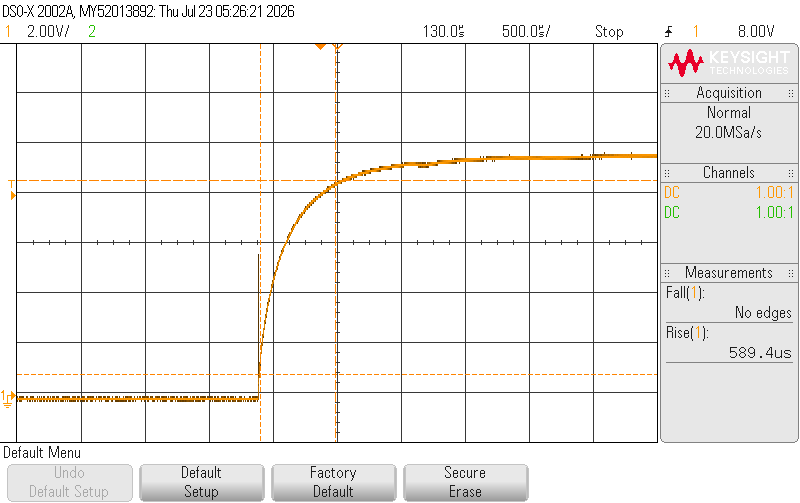
\includegraphics[width=\textwidth]{./figures/scope_5.png}
		\caption{Trial 3}
	\end{subfigure}
	\caption{Oscilloscope captures of the rising step with the coil.}
\end{figure}

\begin{table}[H]
	\centering
	\begin{tabular}{lccc}
		\toprule
		\textbf{Trial} & \textbf{1} & \textbf{2} & \textbf{3} \\
		\midrule
		Rise time & $565.0\,\mu\text{s}$ & $582.8\,\mu\text{s}$ & $589.4\,\mu\text{s}$ \\
		\bottomrule
	\end{tabular}
\end{table}

\pagebreak

\subsection{Falling Step Function without Coil}

\begin{figure}[H]
	\centering
	\begin{subfigure}{0.6\textwidth}
		\centering
		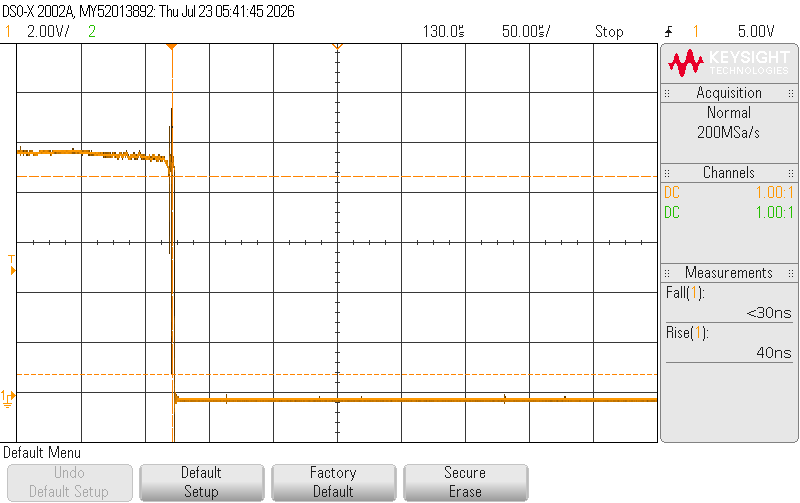
\includegraphics[width=\textwidth]{./figures/scope_9.png}
		\caption{Trial 1}
	\end{subfigure}

	\vspace{0.5em}
	\begin{subfigure}{0.6\textwidth}
		\centering
		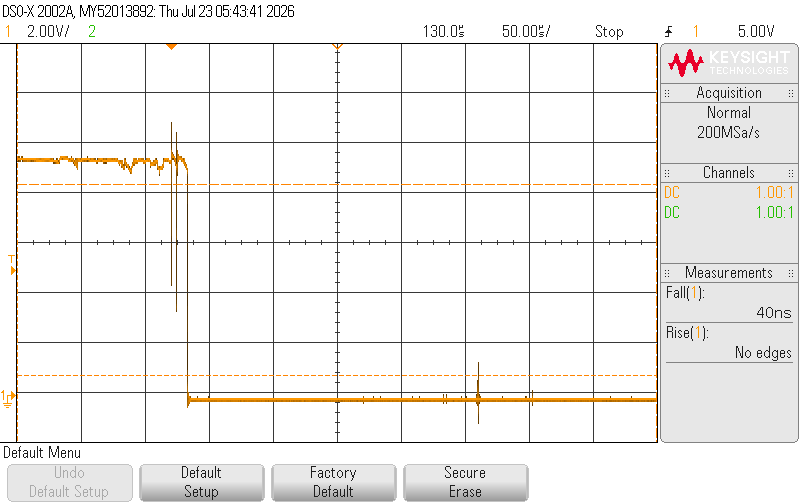
\includegraphics[width=\textwidth]{./figures/scope_10.png}
		\caption{Trial 2}
	\end{subfigure}

	\vspace{0.5em}
	\begin{subfigure}{0.6\textwidth}
		\centering
		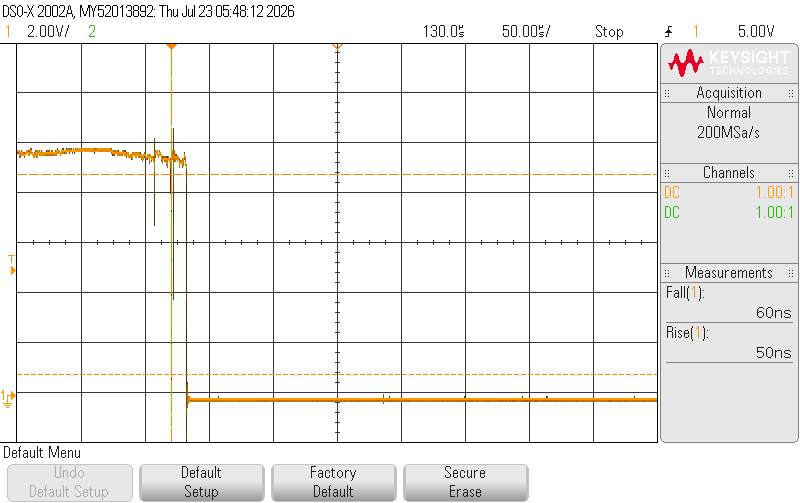
\includegraphics[width=\textwidth]{./figures/scope_12.png}
		\caption{Trial 3}
	\end{subfigure}
	\caption{Oscilloscope captures of the falling step without the coil.}
\end{figure}

\begin{table}[H]
	\centering
	\begin{tabular}{lccc}
		\toprule
		\textbf{Trial} & \textbf{1} & \textbf{2} & \textbf{3} \\
		\midrule
		Fall time & $30\,\text{ns}$ & $40\,\text{ns}$ & $60\,\text{ns}$ \\
		\bottomrule
	\end{tabular}
\end{table}

\pagebreak

\subsection{Falling Step Function with Coil}

\begin{figure}[H]
	\centering
	\begin{subfigure}{0.6\textwidth}
		\centering
		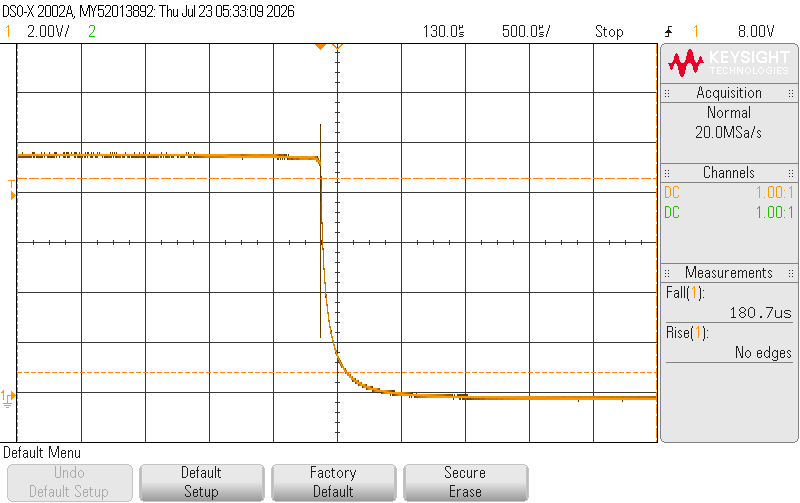
\includegraphics[width=\textwidth]{./figures/scope_6.png}
		\caption{Trial 1}
	\end{subfigure}

	\vspace{0.5em}
	\begin{subfigure}{0.6\textwidth}
		\centering
		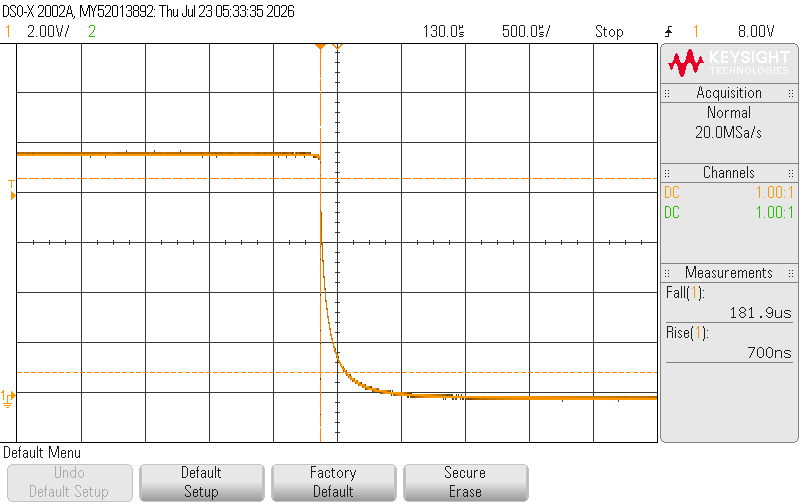
\includegraphics[width=\textwidth]{./figures/scope_7.png}
		\caption{Trial 2}
	\end{subfigure}

	\vspace{0.5em}
	\begin{subfigure}{0.6\textwidth}
		\centering
		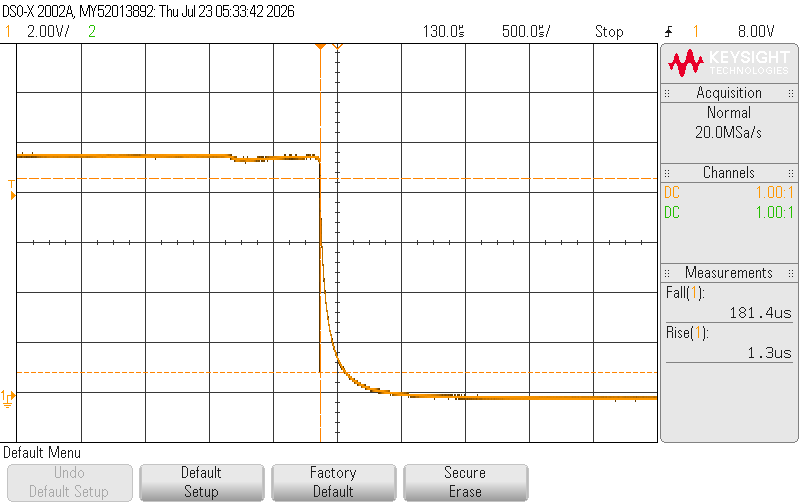
\includegraphics[width=\textwidth]{./figures/scope_8.png}
		\caption{Trial 3}
	\end{subfigure}
	\caption{Oscilloscope captures of the falling step with the coil.}
\end{figure}

\begin{table}[H]
	\centering
	\begin{tabular}{lccc}
		\toprule
		\textbf{Trial} & \textbf{1} & \textbf{2} & \textbf{3} \\
		\midrule
		Fall time & $180.7\,\mu\text{s}$ & $181.9\,\mu\text{s}$ & $181.4\,\mu\text{s}$ \\
		\bottomrule
	\end{tabular}
\end{table}

\end{document}
